\section{Funktioner} \label{Funktioner}
Funktioner defineres som en opgave der skal udføres, og kan yderligere opdeles i delfunktioner (\cite{Ullman2018TheProcess}). Opgaverne der skal udføres i forbindelse med fremstilling af speckle pattern med en robot, illustreres i et flowchart, se figur \ref{fig: flowchart}. Figuren aflæses ved at følge pilene fra en handling til en anden, fra start til slut. 

\begin{figure}[H]
    \centering
    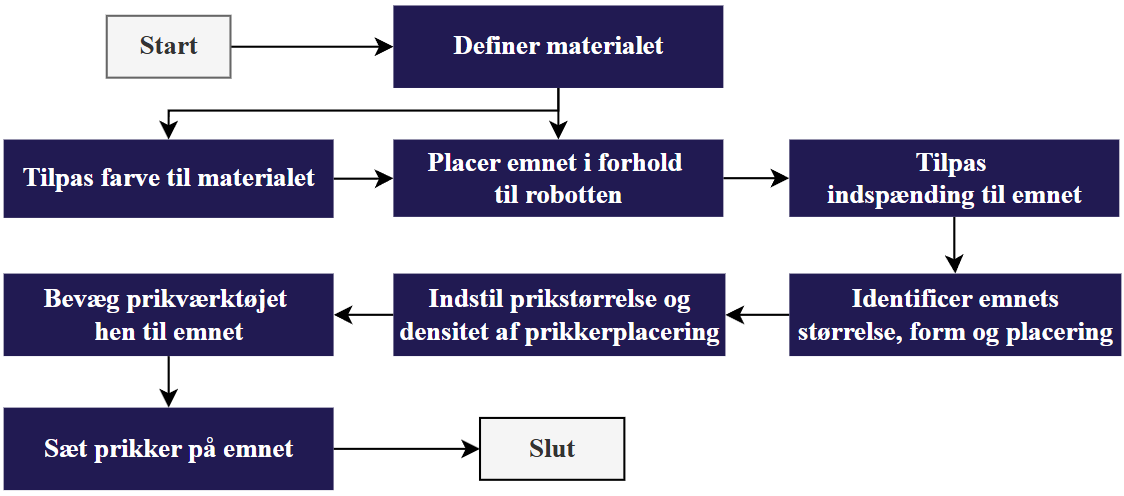
\includegraphics[width=1\linewidth]{Sections/5 Konceptgenerering/Media/Flowchart.png}
    \caption{Flowchart for en robot der skal påsætte speckle patterns}
    \label{fig: flowchart}
\end{figure} \plainbreak{-0.5}

Flowchartet i figur \ref{fig: flowchart} benyttes til at identificere de funktioner og delfunktioner, der ses i figur \ref{Figur: Funktionstræ}. Det er valgt, at opstille alle funktioner i et funktionstræ, for at danne et klart overblik over funktioner og delfunktioner en robot, der sætter speckle patterns skal udføre. Disse benyttes efterfølgende i en morfologisk analyse.  


\newpage
\begin{figure}[H]
\centering
\begin{tikzpicture}
[
    graybox/.style={rectangle, fill=lightgray!20, 
        minimum width=6cm, minimum height=0.8cm, align=center},
    box/.style={rectangle, fill=aaublue, text=white, 
        minimum width=6cm, minimum height=0.8cm, align=center},
    tallbox/.style={rectangle, fill=aaublue, text=white, 
        minimum width=5.8cm, minimum height=1.8cm, align=center, text width=5.8cm},
    arrow/.style={-Stealth, thick}]

% Problemanalyse
\node[tallbox, rotate = 90] (funktioner) {\Large \textbf{Robot til fremstilling af speckle patterns}};

% Funktioner
\node[box, right=1.cm of funktioner.south east, anchor=north west] (bevaegelse) {\textbf{Bevægelse}};
\node[box, below=.8cm of bevaegelse] (kontrolsystem) {\textbf{Kontrolsystem}};
\node[box, below=.8cm of kontrolsystem] (saette) {\textbf{Sætte prikker}};
\node[box, below=.8cm of saette] (fastholde) {\textbf{Fastholde emne}};


%beskrivele Funktion
\node[graybox, above=.2cm of bevaegelse](Funktion){\textbf{Funktioner}};
\draw[lightgray!40, very thick] (1.8,3.1) rectangle (8,-3.2);

%beskrivele delfunktion
\node[graybox, right=1.cm of Funktion](Delfunktion){\textbf{Delfunktioner}};
\draw[lightgray!40, very thick] (8.8,3.1) rectangle (15,-3.2);


% Delfunktioner til Kontrolsystem
\node[box, below=1.3cm of Delfunktion] (brugerflade) {\textbf{Brugerflade}};
\node[box, below=.2cm of brugerflade] (formanalyse) {\textbf{Kalibrering af emne placering}};

% Delfunktioner til Fastholdelse
\node[box, below=1.4cm of formanalyse] (indspaend) {\textbf{Indspænding}};
\node[box, below=.2cm of indspaend] (understot) {\textbf{Understøttelse}};


% Pile
\draw[arrow] (funktioner.south) -- ++(0.5,0) |- (bevaegelse);
\draw[arrow] (funktioner.south) -- ++(0.5,0) |- (saette);
\draw[arrow] (funktioner.south) -- ++(0.5,0) |- (kontrolsystem);
\draw[arrow] (funktioner.south) -- ++(0.5,0) |- (fastholde);

\draw[arrow] (kontrolsystem.east) -- ++(0.5,0) |- (brugerflade);
\draw[arrow] (kontrolsystem.east) -- ++(0.5,0) |- (formanalyse);

\draw[arrow] (fastholde.east) -- ++(0.5,0) |- (indspaend);
\draw[arrow] (fastholde.east) -- ++(0.5,0) |- (understot);

\end{tikzpicture}
\caption{Funktionstræ}
\label{Figur: Funktionstræ}
\end{figure} \plainbreak{-0.5}

Det er valgt ikke at medtage 'tilpas farve til materialet' da der er afgrænset fra farvemidlet i afsnit \ref{Afgrænsning}.


\subsubsection{Bevægelse} \plainbreak{-0.5}
Metode til at flytte prikværktøjet og/eller emnet i forhold til hinanden, der muliggør fremstillingen af et speckle pattern på et 2D plan.



\subsubsection{Kontrolsystem}\plainbreak{-0.5}
%Kontrolsystemet bestemmer hvor og hvornår der skal sættes prikker, og giver feedback til brugeren. Dette er nødvendigt for, at robotten kan påsætte det ønskede speckle pattern, samt give brugeren mulighed for at kunne starte og stoppe maskinen. Kontrolsystemet har to delfunktioner; brugerflade, som skal modtage input og give feedback tilbage til brugeren der betjener robotten og Kalibrering af emnets placering. Kalibreringen er til for, at robotten ved hvor emnet er placeret, dets størrelse og form. For at undgå påsætning af speckle patterns udenfor emnet, er det nødvendig med identifikation af emnets dimensioner.

Det er i afsnit \ref{Afgrænsning} valgt, at afgrænse fra elektronik og software, hvorfor kontrolsystemet ikke medtages i den morfologiske analyse. Det fysiske design af kontrolsystemet har betydning for designet af de mekaniske dele, hvorfor delkoncepter til kontrolsystemet er overfladisk undersøgt i bilag \ref{Bilag - morf til kontrolsystem}.



\subsubsection{Sætte prikker} \plainbreak{-0.5}
En essentiel del af robottens funktion er, at den sætter speckle patterns. Delfunktioner til at sætte prikker vurderes til at være så afhængige af hvilken overordnet metode der bliver valgt, og kan derfor ikke yderligere specificeres, før den overordnede metode er valgt. Dette er fordi løsningerne fra problemanalysens afsnit \ref{DIC afsnit}, har stor variation i metoden til at påsætte prikker og de delfunktioner de kræver. 



\subsubsection{Fastholde emnet} \plainbreak{-0.5}
Emnet skal fastholdes, så emnet ikke flyttes under påsætning af speckle pattern. Fastholdelsen er opdelt i indspænding og understøtning. Emnet må maksimalt flyttes \(\SI{0,01}{mm}\) under påføring af speckle patterns, hvilket nødvendiggør indspænding af emnet, så der ikke sker flytning. Understøtningen defineres som den overflade emnet kan placeres på, hvorefter det kan fastgøres af indspændingen. Understøtningen har til formål at understøtte emnet fra kræfter som tyngdekraften.

%Delfunktionerne til kontrolsystem vurderes at være af minimal betydning for vægtningen af konceptforslagene og afhænger af hvilke mekaniske koncepter der vælges. Der laves derfor først en morfologisk analyse af de mekaniske dele, der omfatter; bevægelse, priksætning, indspænding og understøttelse, efterfulgt af en morfologisk analyse af kontrolsystemet.   

